\documentclass{beamer}
\usepackage[utf8]{inputenc}

\usetheme{Madrid}
\usecolortheme{default}
\usepackage{amsmath,amssymb,amsfonts,amsthm}
\usepackage{txfonts}
\usepackage{tkz-euclide}
\usepackage{listings}
\usepackage{adjustbox}
\usepackage{array}
\usepackage{tabularx}
\usepackage{gvv}
\usepackage{lmodern}
\usepackage{circuitikz}
\usepackage{tikz}
\usepackage{graphicx}

\setbeamertemplate{page number in head/foot}[totalframenumber]

\usepackage{tcolorbox}
\tcbuselibrary{minted,breakable,xparse,skins}



\definecolor{bg}{gray}{0.95}
\DeclareTCBListing{mintedbox}{O{}m!O{}}{%
	breakable=true,
	listing engine=minted,
	listing only,
	minted language=#2,
	minted style=default,
	minted options={%
		linenos,
		gobble=0,
		breaklines=true,
		breakafter=,,
		fontsize=\small,
		numbersep=8pt,
		#1},
	boxsep=0pt,
	left skip=0pt,
	right skip=0pt,
	left=25pt,
	right=0pt,
	top=3pt,
	bottom=3pt,
	arc=5pt,
	leftrule=0pt,
	rightrule=0pt,
	bottomrule=2pt,
	toprule=2pt,
	colback=bg,
	colframe=orange!70,
	enhanced,
	overlay={%
		\begin{tcbclipinterior}
			\fill[orange!20!white] (frame.south west) rectangle ([xshift=20pt]frame.north west);
	\end{tcbclipinterior}},
	#3,
}
\lstset{
	language=C,
	basicstyle=\ttfamily\small,
	keywordstyle=\color{blue},
	stringstyle=\color{orange},
	commentstyle=\color{green!60!black},
	numbers=left,
	numberstyle=\tiny\color{gray},
	breaklines=true,
	showstringspaces=false,
}

\title{Matgeo Presentation - Problem 1.6.11}
\author{EE25BTECH11061 - Vankudoth Sainadh}

\begin{document}

\begin{frame}
  \titlepage
\end{frame}

% Problem Statement
\begin{frame}{Problem Statement}
If the points $A(1,2)$, $O(0,0)$ and $C(a,b)$ are collinear, find the relation between $a$ and $b$.

\end{frame}

% Method
\begin{frame}{Method}
\textbf{Condition for Collinearity:}

Three points $A, O, C$ are collinear iff the collinearity matrix

\begin{align*}
M=\myvec{ \vec{O}-\vec{A} & \vec{C}-\vec{A} }^\top
\end{align*}

has $rank\brak{M}=1$.

\end{frame}

% Part (a)
\begin{frame}{Echelon Form and Row Operations}

\begin{align*}
M &= \big(\,\vec{O}-\vec{A}\;\; \vec{C}-\vec{A}\,\big)^{T}
   = \myvec{-1 & -2\\[4pt] a-1 & b-2},\\
\text{Collinearity} &\iff \operatorname{rank}(M)=1.
\end{align*}

\begin{align*}
R_2 &\longrightarrow R_2 - \frac{a-1}{-1}\,R_1
\quad (\text{note: }-1\neq 0),\\[6pt]
\myvec{-1 & -2\\ a-1 & b-2}
&\longrightarrow
\myvec{-1 & -2\\ 0  & b-2a}.
\end{align*}

\begin{align*}
\operatorname{rank}(M)=1
\;\Longleftrightarrow\;
\text{second row is the zero row}
\;\Longleftrightarrow\;
b-2a=0.
\end{align*}
\begin{align*}
\boxed{\,b=2a\,}.
\end{align*}

\end{frame}


\begin{frame}{Final Answer}

  \begin{center}
 {\LARGE \begin{align*}
   \boxed{b=2a}  
  \end{align*}}
  \end{center}

\end{frame}



% --------- CODE APPENDIX ---------
\section*{Appendix: Code}

% C program
\begin{frame}[fragile]{C Code: points.c }
\begin{lstlisting}[language=C]

#include <stdio.h>

// Function to return relation value  (0 => COLLINEAR)
int relation(int a, int b) {
    return b - 2*a;   // For A(1,2), O(0,0), C(a,b): collinear <=> b - 2a = 0
}

int main(void) {
    // Given points: A(1,2) and O(0,0)
    int x1 = 0, y1 = 0;   // O
    int x2 = 1, y2 = 2;   // A

    // Step 1: Compute slope of line through O and A
    float m = (float)(y2 - y1) / (x2 - x1);
    \end{lstlisting}
\end{frame}

\begin{frame}[fragile]
\begin{lstlisting}[language=C]
    printf("Step 1: Compute slope using two points O(0,0) and A(1,2):\n");
    printf("        m = (y2 - y1) / (x2 - x1) = (%d - %d) / (%d - %d) = %.2f\n\n",
           y2, y1, x2, x1, m);


    // Step 2: Point-slope form using point O(0,0)
    printf("Step 2: Equation using point-slope form (through O):\n");
    printf("        (y - %d) = m (x - %d)\n", y1, x1);
    printf("        => y = m x\n\n");

    // Step 3: Substitute m = 2 (from Step 1)
    printf("Step 3: With m = %.0f, the line is:  y = 2x\n\n", m);
\end{lstlisting}
\end{frame}

\begin{frame}[fragile]
\begin{lstlisting}[language=C]
    // Step 4: Final relation for C(a,b) lying on this line
    printf("Step 4: Substitute C(a,b) into y = 2x  =>  b = 2a\n");
    printf("Final Relation: b - 2a = 0\n\n");

    // (Optional) quick test: uncomment to verify with numbers
    // int a = 3, b = 6;
    // printf("Test with a=%d, b=%d -> residual (b - 2a) = %d\n", a, b, relation(a,b));

    return 0;
}

  
\end{lstlisting}
\end{frame}

% Python calling C
\begin{frame}[fragile]{Python: call\_c.py}
\begin{lstlisting}[language=Python]
import ctypes, argparse

# Load the shared object produced above
lib = ctypes.CDLL("./collinear.so")

# Configure signatures
lib.relation.argtypes = [ctypes.c_int, ctypes.c_int]
lib.relation.restype  = ctypes.c_int

lib.collinear_AO_C.argtypes = [ctypes.c_double, ctypes.c_double, ctypes.c_double,
                               ctypes.POINTER(ctypes.c_double)]
lib.collinear_AO_C.restype  = ctypes.c_int

def main():
    ap = argparse.ArgumentParser(description="Check collinearity for A(1,2), O(0,0), C(a,b)")
    \end{lstlisting}
\end{frame}
\begin{frame}[fragile]
\begin{lstlisting}[language=Python]
    ap.add_argument("--a", type=float, default=3.0)
    ap.add_argument("--b", type=float, default=6.0)
    ap.add_argument("--tol", type=float, default=1e-9)
    args = ap.parse_args()

    # int API (residual = b - 2a as an int)
    r_int = lib.relation(int(round(args.a)), int(round(args.b)))

    # double API (residual + boolean)
    resid = ctypes.c_double()
    ok = lib.collinear_AO_C(args.a, args.b, args.tol, ctypes.byref(resid))

    print(f"Residual (b - 2a) via int API: {r_int}")
    print(f"Residual (b - 2a) via double API: {resid.value:.6e}")
    print("Status:", "COLLINEAR" if ok else "NOT collinear")

if __name__ == "__main__":
    main()

\end{lstlisting}
\end{frame}

% Python plotting
\begin{frame}[fragile]{Python: plot.py }
\begin{lstlisting}[language=Python]
import argparse, os, ctypes
import numpy as np
import matplotlib
if not os.environ.get("DISPLAY"):
    matplotlib.use("Agg")
import matplotlib.pyplot as plt

# load C lib
lib = ctypes.CDLL("./collinear.so")
lib.relation.argtypes = [ctypes.c_int, ctypes.c_int]
lib.relation.restype  = ctypes.c_int

def main():
    ap = argparse.ArgumentParser(description="Plot A(1,2), O(0,0), C(a,b) and line y=2x")
    ap.add_argument("--a", type=float, default=3.0)
    ap.add_argument("--b", type=float, default=6.0)
    \end{lstlisting}
\end{frame}
\begin{frame}[fragile]
\begin{lstlisting}[language=Python]
    ap.add_argument("--save", type=str, default="collinearity_plot.png")
    ap.add_argument("--no-show", action="store_true")
    args = ap.parse_args()

    A = (1.0, 2.0)
    O = (0.0, 0.0)
    C = (args.a, args.b)

    # residual from shared lib (int API, for display)
    r_int = lib.relation(int(round(args.a)), int(round(args.b)))

   # line y = 2x through O and A
    x_min = min(-1.0, O[0], A[0], C[0]) - 0.5
    x_max = max(4.0,  O[0], A[0], C[0]) + 0.5
    xs = np.linspace(x_min, x_max, 400)
    ys = 2 * xs
    plt.figure(figsize=(7,5))
    \end{lstlisting}
\end{frame}

\begin{frame}[fragile]
\begin{lstlisting}[language=Python]
    plt.plot(xs, ys, label="Line through O and A: y = 2x")
    plt.scatter([O[0], A[0], C[0]], [O[1], A[1], C[1]], s=80, marker="x")
   

    plt.text(O[0]+0.05, O[1]+0.05, "O(0,0)")
    plt.text(A[0]+0.05, A[1]+0.05, "A(1,2)")
    plt.text(C[0]+0.05, C[1]+0.05, f"C({C[0]:.3g},{C[1]:.3g})")

    status = "COLLINEAR" if r_int == 0 else "NOT collinear"
    plt.title(f"A, O, C: {status}  (residual b-2a = {r_int})")
    plt.xlabel("x"); plt.ylabel("y"); plt.grid(True); plt.legend(); plt.axis("equal"); plt.tight_layout()

    plt.savefig(args.save, dpi=150)
    print(f"Residual (b - 2a) = {r_int}  ->  {status}")
    print(f"Plot saved to: {args.save}")
\end{lstlisting}
\end{frame}
\begin{frame}[fragile]
\begin{lstlisting}[language=Python]
    if not args.no_show and matplotlib.get_backend().lower() not in {"agg"}:
        plt.show()
if __name__ == "__main__":
    main()

\end{lstlisting}
\end{frame}
\begin{frame}{Plot by python using shared output from c}
	\begin{center}
		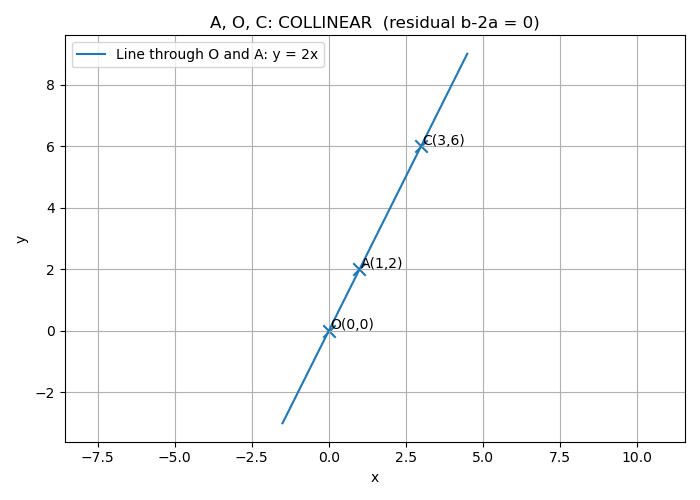
\includegraphics[width=0.6\columnwidth]{figs/Figure_1.png}
	\end{center}
\end{frame}
\end{document}
